\documentclass{standalone}
\begin{document}
\subsection{Aufgabe 12.6}
    \begin{align*}
        M &= \{z\in\mathbb{C}\ |\ |z-3| = 2|z+3|\} \\
          &= \{(a+bi)\in\mathbb{C}\ |\ |(a-3)+bi| = 2|(a+3)+bi|\} \\
          &= \{(a+bi)\in\mathbb{C}\ |\ \sqrt{(a-3)^2+b^2} = 2\sqrt{(a+3)^2+b^2}\} \\
          &= \{(a+bi)\in\mathbb{C}\ |\ a^2-6a+9+b^2 = 4(a^2+6a+9+b^2)\} \\
          &= \{(a+bi)\in\mathbb{C}\ |\ -3a^2-30a-27 = 3b^2\} \\
          &= \{(a+bi)\in\mathbb{C}\ |\ b^2 = -a^2-10a-9\} \\
    \end{align*}

    \begin{center}
        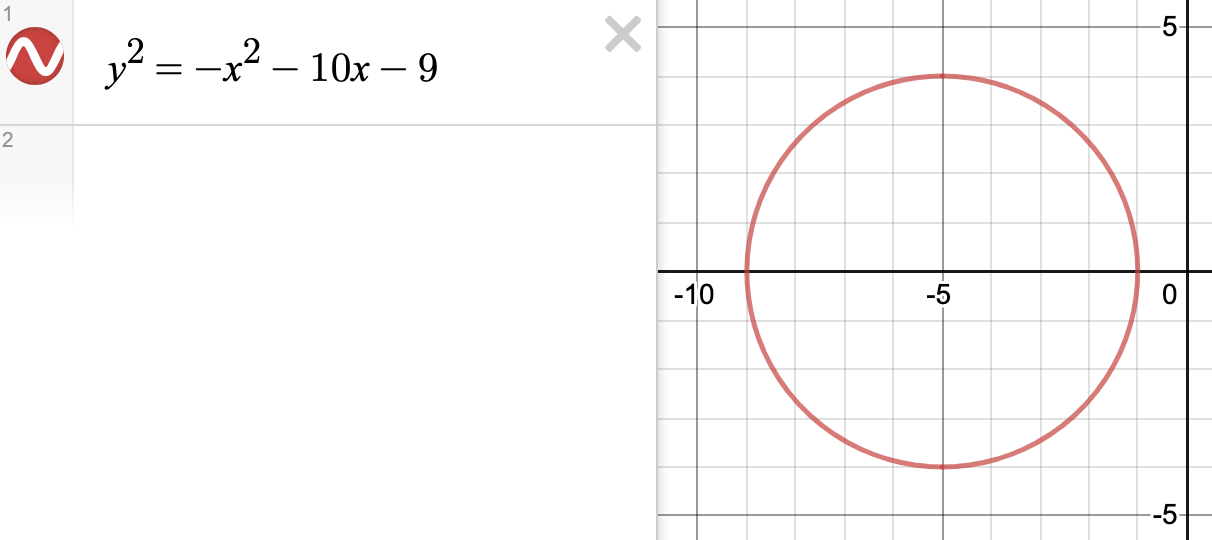
\includegraphics[width=10cm]{img/12_6.png}
    \end{center}

    $\therefore$ Die Menge der komplexen Zahlen $M$ bildet einen Kreis in der komplexen Ebene.

\end{document}
